\documentclass[tikz]{standalone}
\usepackage{tkz-graph}
\usepackage{amsmath,amssymb}
\usepackage{xcolor}
\usetikzlibrary{calc}
\usetikzlibrary{positioning}
\usepackage{pgfplots}

\pgfplotsset{compat=newest}
\usepgfplotslibrary{fillbetween}

\begin{document}


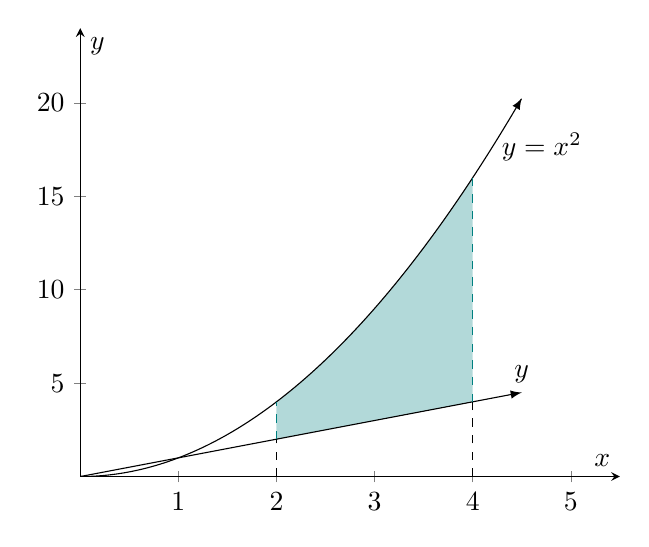
\begin{tikzpicture}


	\begin{axis}[axis lines = middle, xlabel = {\(x\)}, ylabel = {\(y\)},
			xmin=0, xmax=5.5, ymin=0, ymax=24]

		\addplot [name path = A, -latex, domain=0:4.5, samples =1000] {x^2}
		node [very near end, right] {\(y=x^2\)};

		\addplot [name path =B, -latex, domain = 0:4.5]{x} node[pos=1, above] {\(y\) };
		\addplot [teal!30] fill between [of = A and B, soft clip ={domain=2:4}];


		\draw [dashed, teal] (axis cs:{2,2}) -- (axis cs:{2,4});
		\draw [dashed, teal] (axis cs:{4,4}) -- (axis cs:{4,16});
		\draw [dashed] (axis cs:{2,0}) -- (axis cs:{2,2});
		\draw [dashed] (axis cs:{4,0}) -- (axis cs:{4,4});

	\end{axis}

\end{tikzpicture}

\end{document}

